%%%%%%%%%%%%%%%%%%%%%%%%%%%%%%%%%%%%%%%%%%%%%%%%%%%%%%%%%%%%%%%%%%%%%%%%%%%%%%%%% Conformal Killing Spinor Initial Data Equations. CENTRA-CAMGSD 2022.
%%%%%%%%%%%%%%%%%%%%%%%%%%%%%%%%%%%%%%%%%%%%%%%%%%%%%%%%%%%%%%%%%%%%%%%%%%%%%%%%% 


% Pour la presentation:
\documentclass[10pt]{beamer}

% Pour la diffusion du document PDF:
%\documentclass[10pt,handout]{beamer}

\mode<presentation>
{
  \usetheme{Warsaw}
%\usecolortheme{dolphin}
 
  %\usetheme{default}
  % or ...

  \setbeamercovered{transparent}
  %\setbeamercovered{invisible}
  % or whatever (possibly just delete it)
}

%\usepackage[french]{babel}
% or whatever

\usepackage[latin1]{inputenc}
% or whatever


%\usepackage{times}
%\usepackage[T1]{fontenc}
% Or whatever. Note that the encoding and the font should match. If T1
% does not look nice, try deleting the line with the fontenc.

\usepackage{bm}                  % bold math
\usepackage{amssymb,amsfonts}    % AMS Symbols
\usepackage{amsthm}              %AMS theorems
\usepackage{mathrsfs}
%\usepackage{color}
\usepackage[dvipsnames]{color}
\hypersetup{pdfstartview=Fit,pdfpagelayout=SinglePage,pdfpagemode=None}
\usepackage{xcolor}
%%%%% to cancel terms %%%%%%%%%
\usepackage{cancel}
%%%%%%%%%%%%%%%%

%\usepackage{mathtools,graphicx}
%\newcommand\vertarrowbox[2]{%
%    \begin{array}[t]{@{}c@{}} #1 \\
%    \rotatebox{90}{$\xrightarrow{\hphantom{abcdefgh}}$} \\[-1ex]
%    \mathclap{\scriptstyle\text{#2}}%
%    \end{array}}



\title[CKSID] % (optional, use only with long paper titles)
{The conformal Killing spinor initial data equations
}
\author{Edgar Gasper\'in}
\titlegraphic{
  \vspace{-10mm}
  
\includegraphics[width=2cm]{figs/centra.png}
  \hfill{}
  \vspace{\fill}  
  
\includegraphics[width=3.3cm]{figs/camgsd.png}%{figs/centra.png}

}



\institute[CENTRA-IST] % (optional, but mostly needed)
{\alert{

\textcolor{black}{{\normalsize{
in collaboration with  Jarrod L. Williams   \\ \medskip
arXiv:1704.07586v2 [gr-qc]. To appear in Journal of Geometry and Physics  }}}\\ \medskip
{} \\
} \\
[1ex]
\href{mailto:edgar.gasperin@tecnico.ulisboa.pt}{\blue{edgar.gasperin@tecnico.ulisboa.pt}}}

% - Use the \inst command only if there are several affiliations.
% - Keep it simple, no one is interested in your street address.

%\date[CFP 2003] % (optional, should be abbreviation of conference name)
%{Conference on Fabulous Presentations, 2003}
\date[]
{23 June 2022\\
@ Joint seminar CENTRA-CAMGSD 
}
% - Either use conference name or its abbreviation.
% - Not really informative to the audience, more for people (including
%   yourself) who are reading the slides online

%\subject{}
% This is only inserted into the PDF information catalog. Can be left

% out. 

% If you have a file called "university-logo-filename.xxx", where xxx
% is a graphic format that can be processed by latex or pdflatex,
% resp., then you can add a logo as follows:

% \pgfdeclareimage[height=0.5cm]{university-logo}{university-logo-filename}
% \logo{\pgfuseimage{university-logo}}

%\usecolortheme{seahorse}
%\usefonttheme[onlymath]{serif}
\setbeamercolor{math text}{fg=blue}

% Delete this, if you do not want the table of contents to pop up at
% the beginning of each subsection:
\AtBeginSubsection[]
{
  \begin{frame}<beamer>
    \frametitle{Outline}
    \tableofcontents[currentsection,currentsubsection]
  \end{frame}
}

\AtBeginSection[]
{
  \begin{frame}<beamer>
    \frametitle{Outline}
    \tableofcontents[currentsection]
  \end{frame}
}


% If you wish to uncover everything in a step-wise fashion, uncomment
% the following command: 
%\beamerdefaultoverlayspecification{<+->}

%%%%%%%%%%%%%%%%%%%%%%%%%%%%
% Perso:
%\usecolortheme{crane}
\usefonttheme[onlymath]{serif}
%\usefonttheme{structurebold}
\useoutertheme{infolines}
%\setbeamercolor{math text}{fg=blue}
\let\gm\gamma
% Scri
\font\svtnscr=rsfs10 scaled1700
\font\tenscr=rsfs10 scaled1100
\font\sevenscr=rsfs7 % scaled \magstep1
\font\fivescr=rsfs5 % scaled \magstep1
\skewchar\tenscr='177
\skewchar\sevenscr='177
\skewchar\fivescr='177
\newfam\scrfam
\textfont\scrfam=\tenscr
\scriptfont\scrfam=\sevenscr
\scriptscriptfont\scrfam=\fivescr
\def\scr{\fam\scrfam}

\newcommand{\SCRI}{{\svtnscr I}}
\newcommand{\Scri}{{\tenscr I}}
\def\scri{{\fam\scrfam I}}
\def\scrm{{\fam\scrfam M}}
\def\scru{{\fam\scrfam U}}
\def\scrc{{\fam\scrfam C}}

%% Complex and real numbers
%\font\SYM=msbm10 scaled1700
\font\SYM=msbm10 scaled1100
\newcommand{\Real}{{\SYM R}}
\newcommand{\Complex}{{\SYM C}}
\newcommand{\Natural}{{\SYM N}}
\newcommand{\Sphere}{{\SYM S}}

\def\blue{\textcolor{blue}}
\def\black{\textcolor{black}}
\def\green{\textcolor{green}}
\def\white{\textcolor{white}}
\def\orange{\textcolor{orange}}
\def\yellow{\textcolor{yellow}}
%\def\gr#1{\textcolor[named]{ForestGreen}{#1}}
\def\gr{\textcolor{ForestGreen}}

\def\pb{p_\bullet}



\theoremstyle{plain}
 \newtheorem{proposition}{Proposition} 
% \newtheorem{lemma}{Lemma}
% \newtheorem{theorem}{\textcolor{blue}{Theorem}}
% \newtheorem*{assumptions}{Assumptions}
\newtheorem*{conjecture}{Conjecture}
% \newtheorem*{subconjecture}{Subconjecture}
% \newtheorem{corollary}{Corollary}
\newtheorem*{main}{Theorem}
%\newtheorem*{definition}{Definition}
% \newtheorem*{proposal}{\textcolor{blue}{Proposal}}

\newcommand{\deuxcol}[4]{\begin{columns}
    \begin{column}{#1\textwidth}#3\end{column}
    \begin{column}{#2\textwidth}#4\end{column}
        \end{columns}}


% Boldface mathmode lowcase latin letters
\def\bma{{\bm a}}
\def\bmb{{\bm b}}
\def\bmc{{\bm c}}
\def\bmd{{\bm d}}
\def\bme{{\bm e}}
\def\bmf{{\bm f}}
\def\bmg{{\bm g}}
\def\bmh{{\bm h}}
\def\bmi{{\bm i}}
\def\bmj{{\bm j}}
\def\bmk{{\bm k}}
\def\bml{{\bm l}}
\def\bmn{{\bm n}}
\def\bmm{{\bm m}}
\def\bmo{{\bm o}}
\def\bmq{{\bm q}}
\def\bms{{\bm s}}
\def\bmt{{\bm t}}
\def\bmu{{\bm u}}
\def\bmv{{\bm v}}
\def\bmw{{\bm w}}
\def\bmx{{\bm x}}
\def\bmy{{\bm y}}
\def\bmz{{\bm z}}

% Boldface mathmode numbers
\def\bmzero{{\bm 0}}
\def\bmone{{\bm 1}}
\def\bmtwo{{\bm 2}}
\def\bmthree{{\bm 3}}

% Boldface mathmode uppercase latin letters
\def\bmA{{\bm A}}
\def\bmB{{\bm B}}
\def\bmC{{\bm C}}
\def\bmD{{\bm D}}
\def\bmE{{\bm E}}
\def\bmF{{\bm F}}
\def\bmG{{\bm G}}
\def\bmH{{\bm H}}
\def\bmK{{\bm K}}
\def\bmL{{\bm L}}
\def\bmM{{\bm M}}
\def\bmN{{\bm N}}
\def\bmP{{\bm P}}
\def\bmQ{{\bm Q}}
\def\bmR{{\bm R}}
\def\bmS{{\bm S}}
\def\bmT{{\bm T}}
\def\bmX{{\bm X}}
\def\bmZ{{\bm Z}}

\def\Riem{{\bm R}{\bm i}{\bm e}{\bm m}}
\def\Ric{{\bm R}{\bm i}{\bm c}}
\def\Weyl{{\bm W}{\bm e}{\bm y}{\bm l}}
\def\RWeyl{{\bm R}{\bm W}{\bm e}{\bm y}{\bm l}}
\def\Sch{{\bm S}{\bmc}{\bm h}}
\def\Schouten{{\bm S}{\bmc}{\bm h}{\bm o}{\bm u}{\bm t}{\bm e}{\bm n}}
\def\Hessian{{\bm H}{\bm e}{\bm s}{\bm s}}

% Fracture letters
\def\fraka{{\frak a}}
\def\frakb{{\frak b}}
\def\frakc{{\frak c}}
\def\fraki{{\frak i}}
\def\frakj{{\frak j}}
\def\frakk{{\frak k}}

% Mathbf letters
\def\mbfu{\mathbf{u}}

% Boldface mathmode lowcase greek letters
\def\bmalpha{{\bm \alpha}}
\def\bmbeta{{\bm \beta}}
\def\bmgamma{{\bm \gamma}}
\def\bmdelta{{\bm \delta}}
\def\bmepsilon{{\bm \epsilon}}
\def\bmeta{{\bm \eta}}
\def\bmzeta{{\bm\zeta}}
\def\bmxi{{\bm \xi}}
\def\bmchi{{\bm \chi}}
\def\bmiota{{\bm \iota}}
\def\bmomega{{\bm \omega}}
\def\bmlambda{{\bm \lambda}}
\def\bmmu{{\bm \mu}}
\def\bmnu{{\bm \nu}}
\def\bmphi{{\bm \phi}}
\def\bmvarphi{{\bm \varphi}}
\def\bmsigma{{\bm \sigma}}
\def\bmvarsigma{{\bm \varsigma}}
\def\bmtau{{\bm \tau}}
\def\bmupsilon{{\bm \upsilon}}

% Boldface mathmode uppercase greek letters
\def\bmGamma{{\bm \Gamma}}
\def\bmPhi{{\bm \Phi}}
\def\bmUpsilon{{\bm \Upsilon}}
\def\bmSigma{{\bm \Sigma}}

% Boldface operators
\def\bmpartial{{\bm \partial}}
\def\bmnabla{{\bm \nabla}}
\def\bmhbar{{\bm \hbar}}
\def\bmperp{{\bm \perp}}
\def\bmell{{\bm \ell}}

\begin{document}

%%%%% Title slide %%%%

\begin{frame}
  \titlepage
\end{frame}

%% %%%%%%%%%%%%%%%%%

%% \begin{frame}{Plan for the talk}


%% \begin{alertblock}{General aim}
%% \item{ Exploit conformal methods for the analysis of global properties of solutions to the Einstein field equations.}
%% \end{alertblock}


%% \begin{itemize}


%% \item  Introduction and general notions:
%%  Symmetries in GR and the Cauchy problem 
%% \pause
%% \medskip

%% \item The main tool: The conformal Einstein field equations

%% \pause
%% \medskip
%% \item The main result: The conformal Killing spinors initial data equations

%% \end{itemize}
%% %\pause
%% %\begin{exampleblock}{Remark:}
%% %The analysis of the SdS spacetime is a \textbf{model problem} in
%% %  which to develop techniques for more complicated spacetimes.
%% %\end{exampleblock}

%% \end{frame}

%% %%%%%%%%%%%%

%% \section{Symmetries in GR and the Cauchy problem}

%% %%%%%%%%%%%

\begin{frame}
\frametitle{Spinorial notation in a nutshell}
Translation spinors and world tensors $a\rightarrow AA'$.
%\pause
Given $T_{\bma\bmb}$ the spinorial counterpart is given by
\begin{equation*}
T_{\bmA\bmA'\bmB\bmB'}=T_{\bma\bmb}\sigma^{\bma}{}_{\bmA\bmA'}\sigma^{\bmb}{}_{\bmB\bmB'}
\end{equation*} 
where $\sigma^{\bma}{}_{\bmA\bmA'}$ are the Infeld-van der Waerden symbols (Pauli matrices \& Identity) 
%\pause
\begin{equation*}
(\alpha_{\bm0},\alpha_{\bm1},\alpha_{\bm2},\alpha_{\bm3})\rightarrow
\frac{1}{\sqrt{2}}
  \begin{bmatrix}
    \alpha_{\bm0}+ \alpha_{\bm3} & \alpha_{\bm1}-\mbox{i}\alpha_{\bm2} \\
    \alpha_{\bm1}+\mbox{i}\alpha_{\bm2} &  \alpha_{\bm0}-\alpha_{\bm3}
  \end{bmatrix}
\end{equation*}
\pause
\vspace{2mm}
\[
\text{ \textcolor{black}{(frame-) metric:}}\quad g_{AA'BB'}=\epsilon_{AB}\epsilon_{A'B'}
\]
\[
\text{\textcolor{black}{Raise and lower indices:}}\quad \xi_{B}=\xi^A\epsilon_{AB}
\]
%Irreducible decomposition, e.g., $Y_{abc}=Y_{[ab]c}$
%\[
%Y_{abc}\mapsto  Y_{ABCC'}\epsilon_{A'B'} + Y_{AA'BB'CC'}=\bar{Y}_{A'B'C'C}\epsilon_{AB}
%\]
%where $Y_{ABCC'}\equiv \frac{1}{2}Y_{(A|Q'|B)}{}^{Q}{}_{CC'}$.\\
\begin{center}
Curvature spinors:\\
Riemann $\rightarrow$ Weyl, \;\;\;tracefree Ricci, \;\;\; Ricci scalar.
\end{center}
\[
\Psi_{ABCD}, \qquad \Phi_{ABA'B'}, \qquad \Lambda
\]
%\[
%C_{AA'BB'CC'DD'}=\bar{\Psi}_{A'B'C'D'}\epsilon_{AB}\epsilon_{CD}+\Psi_{ABCD}\epsilon_{A'B'}\epsilon_{C'D'}
%\]
%Commutator of covariant derivatives and curvature:
%\[ [\nabla_{a},\nabla_{b}]\kappa^{c}\equiv\nabla_{a}\nabla_{b}\kappa^c-\nabla_{b}\nabla_{a}\kappa^c=R_{ab}{}^{c}{}_{d}\kappa^{d}.\]
%\vspace{-2mm}
%\pause
%\[
%[ \nabla_{AA'},\nabla_{BB'}]= \epsilon_{AB}\square_{A'B'} +
%\epsilon_{A'B'}\square_{AB}
%\]
%where
%\vspace{-3mm}
%\[ \quad
%g_{AA'BB'}=\epsilon_{AB}\epsilon_{A'B'},\quad \square_{AB} \equiv \nabla_{Q'(A} \nabla_{B)}{}^{Q'} \qquad \square \equiv \nabla_{AA'}\nabla^{AA'}
%\]
%\pause
%\begin{equation*}
%\square_{AB}\xi_{C}=-\Psi_{ABCD} \xi^{D} +
%  2\Lambda\xi_{(A}\epsilon_{B)C},
% \label{SpinorialRicciIdentities1} 
%\qquad \square_{A'B'}\xi_{C}=-\xi^{A}\Phi_{CA A' B'},
%\label{SpinorialRicciIdentities2}
%\end{equation*}
%\pause
%\begin{equation*}\label{DecomposeDoubleDerivativeContracted}
%\nabla_{AQ'}\nabla_{B}{}^{Q'}=\square_{AB}+
%\frac{1}{2}\epsilon_{AB}\square
%\end{equation*}
\end{frame}

\begin{frame}
\frametitle{Killing spinors: Hidden symmetries}
\begin{columns}
\column{7.3cm}
\vspace{-4mm}
\onslide<1->
\begin{block}{ Some Killing objects }
\begin{itemize}
\item Killing vectors \[\tilde{\nabla}_{(a}\tilde{\xi}_{b)}=0.
  %\quad \tilde{u}^{a}\tilde{\nabla}_{a}\tilde{u}^{b}=0, \quad E=\tilde{\xi}_{a}\tilde{u}^{a}
  \]
\vspace{-5mm}
\onslide<2->
 \item Killing tensors
   \[ \tilde{K}_{ab}=\tilde{K}_{(ab)},\quad \tilde{\nabla}_{(a}\tilde{K}_{bc)}=0,
   %\quad C=\tilde{K}_{ab}\tilde{u}^{a}\tilde{u}^{b}
   \]
 %  \vspace{-5mm}
 %  \[
 %   \tilde{\zeta}_{b}=\tilde{\xi}^{a}\tilde{K}_{ab}.
 %  \]
\vspace{-5mm}
\onslide<3->
\item Killing-Yano tensors
\[\tilde{Y}_{ab}=\tilde{Y}_{[ab]}, \quad \tilde{\nabla}_{(a}\tilde{Y}_{b)c}=0,\]
\vspace{-5mm}
 \[
 \tilde{K}_{ab}=\tilde{Y}_{a}{}^{c}\tilde{Y}_{cb}.
\]
\vspace{-5mm}
\onslide<4->
\item Killing spinors 
\vspace{-2mm}
\[\tilde{\kappa}_{AB}=\tilde{\kappa}_{(AB)}, \quad \tilde{\nabla}_{A'(A}\tilde{\kappa}_{BC)}=0\]
\vspace{-5mm}
\[ \tilde{Y}_{AA'BB'}=\mbox{i}(\tilde{\kappa}_{AB}\tilde{\epsilon}_{A'B'} - \bar{\tilde{\kappa}}_{A'B'}\tilde{\epsilon}_{AB}) \]
\textcolor{red}{\quad Killing spinors are more primitive objects!}
\end{itemize}
\end{block}
\column{4.3cm}
\vspace{-4mm}
\onslide<2->
\begin{block}{An example: Kerr spacetime}
\[ \tilde{\xi}^{a}=(\partial_{t})^a, \hspace{1mm} \tilde{\eta}^{a}
=(\partial_{\varphi})^{a},\] \[  \exists \tilde{K}_{ab}, \qquad \tilde{u}^{a}\tilde{\nabla}_{a}\tilde{u}^b=0.
%\quad \tilde{\zeta}^{a}=a^2(\partial_{t})^a+a(\partial_{\varphi})^{a}
\]
\[\mu=\tilde{u}^{a}\tilde{u}_{a}, \quad e=\tilde{\xi}^a\tilde{u}_{a},\]\[\ell=\tilde{\eta}^{a}\tilde{u}_{a}, \quad  C=\tilde{K}_{ab}\tilde{u}^a\tilde{u}^b\]
\end{block}
\vspace{2mm}
\begin{alertblock}{Observations}
\begin{itemize}
\item Geodesic motion completely integrable!
\item Hidden symmetry %: $K_{ab}$ not written as a tensor product of Killing vectors
\end{itemize}
\end{alertblock}
\end{columns}
\end{frame}
%%%%%%%%%%%


%%%%%%%%%%%%%%%%%%

\begin{frame}
\frametitle{Rigidity thru symmetries. Symmetries thru intial data}
\begin{columns}
\column{7.3cm}
\vspace{-4mm}
\onslide<1->
\begin{block}{Spacetime symmetries }
\begin{itemize}
\item Black hole uniqueness problems
\item Spacetime characterisations
\end{itemize}
\end{block}
%% \begin{exampleblock}{Petrov Type}
%%   \begin{itemize}
%% \item $\exists$ $\tilde{\kappa}_{AB}$ on $(\tilde{\mathcal{M}},\tilde{\bmg})$
%%   $\implies$ $(\tilde{\mathcal{M}},\tilde{\bmg})$ is  D, N, O.
%%   \end{itemize}
%% \end{exampleblock}
\begin{block}{Killing Initial Data KIDs (Chrusciel \& Beig 97)}
  \begin{itemize}
  \item
    Given initial data $(\tilde{\Sigma},\tilde{h}_{ij},\tilde{\chi}_{ij})$
    for the \textbf{vacuum \underline{Einstein} Field Equations} (EFE)
    if the \textbf{Killing \underline{vector} initial data equations} (KID) are satisfied on $\tilde{\Sigma}$ then the spacetime developement  admits a Killing vector $\xi^a$.
%  \item  $\tilde{\xi}^a=\xi n^a + \zeta^a$.
%  \item KIDs constraint eqs for
%    $(\xi,\zeta^i)$ on $\tilde{\mathcal{S}}$.
\end{itemize}
\end{block}
\column{4.3cm}
\begin{figure}
  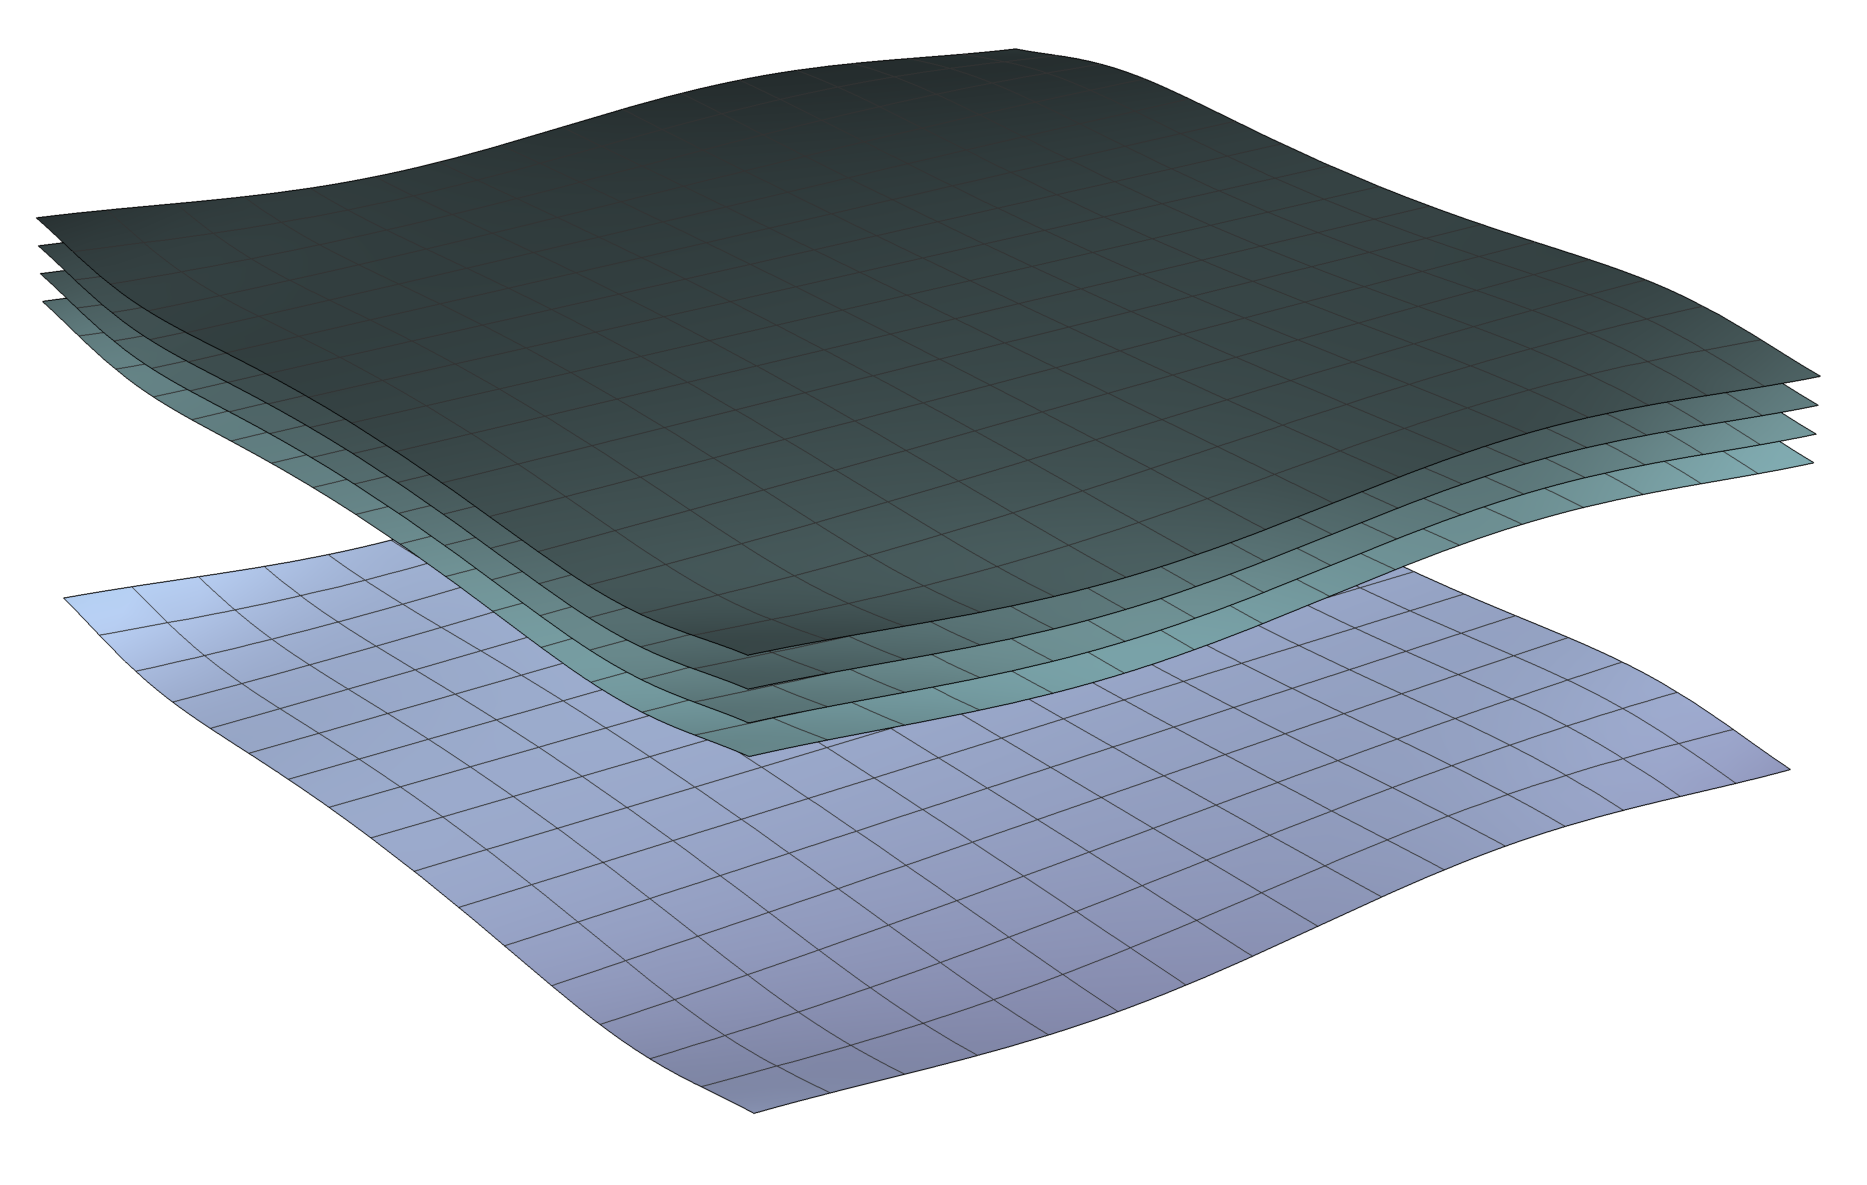
\includegraphics[width=1.05\textwidth]{figs/foliation.png}
  \put(-75,15){\large{$\color{white}\tilde{\Sigma}$}}
  \put(-75,48){\large{$\color{white}\mathcal{\tilde{M}}$}}
%\put(-85,48){\large{$\color{blue}\mathcal{D}^{+}(\tilde{\Sigma})$}}
\end{figure}
\end{columns}
\end{frame}
%%%%%%%%%%%





%%%%%%%%%%%%%%%%%%%




\begin{frame}
\begin{columns}
\column{6.5cm}
\frametitle{Killing vector initial data}
\vspace{-5mm}
\onslide<1->
\begin{exampleblock}{KID: Killing vector initial data }
  \begin{itemize}
  \item Let $(\tilde{\mathcal{M}},\tilde{\bmg})$ solution to $\tilde{R}_{ab}=0$.
  %\item
    \[\tilde{S}_{ab} := \tilde{\nabla}_{a}\tilde{\xi}_{b}+\tilde{\nabla}_{b}\tilde{\xi}_{a}\]
    \vspace{-5mm}
  \item $\tilde{\xi}_{a}$ is KV iff $\tilde{S}_{ab}=0$ (zero-quantity)
  \item Does $\tilde{S}_{ab}=0$ propagate?
    %  \\   i.e. $\tilde{S}_{ab}|_{\tilde{\Sigma}}=0$ $\implies$ $S_{ab}=0$ on
    % $\mathcal{D}^{+}{\tilde{\Sigma}}$??
  %% \onslide<4->\item Yes!
  %%   Trivial data: $\tilde{S}_{ab}=0$ \& $\partial_t \tilde{S}_{ab}=0$ on $\tilde{\Sigma}$  $\implies$ ($\tilde{\xi}_a, \partial_t \tilde{\xi}_a$) on $\tilde{\Sigma}$  aka KIDs.
  \end{itemize}
\end{exampleblock}
\vspace{-2mm}
%\onslide<4->
%\begin{alertblock}{ KIDs}
%  Trivial $\tilde{S}_{ab}$ data  $\leadsto$ ($\tilde{\xi}_a, \partial_t \tilde{\xi}_a$)
%on $\tilde{\Sigma}$  aka KIDs.
%  \end{alertblock}
\column{5.3cm}
\vspace{-5mm}
\onslide<3->
\begin{block}{Identities to eqs}
  \begin{itemize}
   \item Assume \textbf{vacuum EFE} $\qquad \quad \tilde{R}_{ab}=0$
   \item Assume \textbf{candidate} eqn $\tilde{\square}\tilde{\xi}_a=0$ on $(\tilde{\mathcal{M}},\tilde{\bmg})$
   \item  $\implies$ Propagation equation
     \vspace{-2mm}
     \[
     \tilde{\square}\tilde{S}_{ab}=2\tilde{R}^{c}{}_{ab}{}^{d}\tilde{S}_{cd}
     \]
     \vspace{-7mm}
   \item $\tilde{S}_{ab}=0$ \& $\partial_t \tilde{S}_{ab}=0$ on $\tilde{\Sigma}$
     $\implies$ $\tilde{S}_{ab}=0$ on $\mathcal{W}\subseteq\mathcal{D}^{+}(\tilde{\Sigma})$
  \end{itemize}
\end{block}
\end{columns}
\onslide<2->
\begin{block}{Sketch of the KIDs derivation \& proof}
  \begin{itemize}
  \item Identity:
    \vspace{-3mm}
  %\item identities:
      \[\tilde{\nabla}^a\tilde{S}_{ab}-\frac{1}{2}\nabla_b S_{a}{}^{a}=\tilde{\square} \tilde{\xi}_b + \tilde{R}_{cb}\]
      \vspace{-5mm}
      \item Definition: A \textbf{candidate} KV $\tilde{\zeta}^a$ is a vector
        satisfying $\tilde{\square}\tilde{\zeta}_a=-\tilde{R}_{ab}\tilde{\zeta}^b$
        %\item All KV is a candidate but not all candidate is a KV.
        %\vspace{-5mm}
      \item Strategy: find ID ($\zeta_a, \partial_t \zeta_a$) on $\tilde{\Sigma}$
        ensuring a \textbf{candidate} gives a \textbf{true KV}.
      \item  Indentity:
        \vspace{-5mm}
         \[ \tilde{\square}\tilde{S}_{ab}=2\tilde{R}^{c}{}_{ab}{}^{d}\tilde{S}_{cd}-\mathcal{L}_{\tilde{\xi}}\tilde{R}_{ab} +
     2 \tilde{\nabla}_{(a}\left\{\tilde{\square}\tilde{\xi}_{b)} +\tilde{R}_{b{)}c}\tilde{\xi}^c\right\}\]
     \vspace{-5mm}
        \end{itemize}   
\end{exampleblock}
\end{frame}



\begin{frame}
\begin{columns}
\column{6.5cm}
\frametitle{Killing vector initial data}
\vspace{-5mm}
\begin{exampleblock}{KID: Killing vector initial data }
  \begin{figure}
    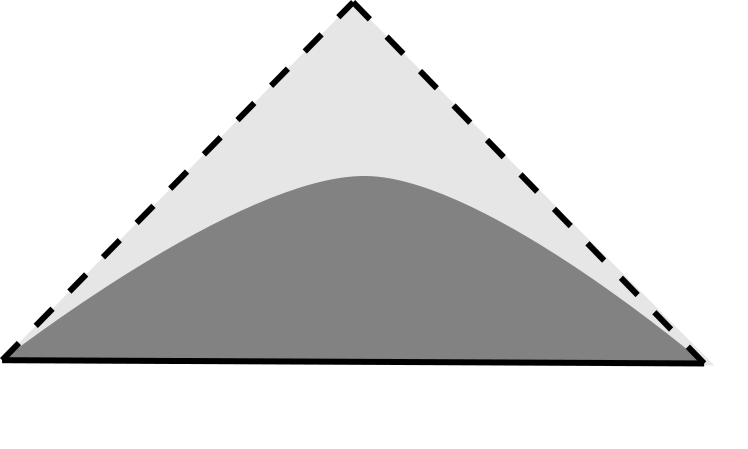
\includegraphics[width=0.9\textwidth]{figs/DomainDependece.png}
  \put(-94,22){\large{$\color{blue}\tilde{\Sigma}$}}
  \put(-94,45){\large{$\color{blue}\mathcal{W}$}}
\put(-105,70){\large{$\color{blue}\mathcal{D}^{+}(\tilde{\Sigma})$}}
  \end{figure}
  \vspace{-8mm}
  Trivial data: $\tilde{S}_{ab}=0$ \& $\partial_t \tilde{S}_{ab}=0$ on $\tilde{\Sigma}$
  $\implies$ ($\tilde{\xi}_a, \partial_t \tilde{\xi}_a$) on $\tilde{\Sigma}$  aka KIDs.
\end{exampleblock}
\vspace{-2mm}
\column{5.3cm}
\vspace{-5mm}
\begin{block}{Identities to eqs}
  \begin{itemize}
   \item Assume \textbf{vacuum EFE} $\qquad \quad \tilde{R}_{ab}=0$
   \item Assume \textbf{candidate} eqn $\tilde{\square}\tilde{\xi}_a=0$ on $(\tilde{\mathcal{M}},\tilde{\bmg})$
   \item  $\implies$ Propagation equation
     \vspace{-2mm}
     \[
     \tilde{\square}\tilde{S}_{ab}=2\tilde{R}^{c}{}_{ab}{}^{d}\tilde{S}_{cd}
     \]
     \vspace{-7mm}
   \item $\tilde{S}_{ab}=0$ \& $\partial_t \tilde{S}_{ab}=0$ on $\tilde{\Sigma}$
     $\implies$ $\tilde{S}_{ab}=0$ on $\mathcal{W}\subseteq\mathcal{D}^{+}(\tilde{\Sigma})$
  \end{itemize}
\end{block}
\end{columns}
\begin{block}{Sketch of the KIDs derivation \& proof}
  \begin{itemize}
  \item Identity:
    \vspace{-3mm}
      \[\tilde{\nabla}^a\tilde{S}_{ab}-\frac{1}{2}\nabla_b S_{a}{}^{a}=\tilde{\square} \tilde{\xi}_b + \tilde{R}_{cb}\]
      \vspace{-5mm}
      \item Definition: A \textbf{candidate} KV $\tilde{\zeta}^a$ is a vector
        satisfying $\tilde{\square}\tilde{\zeta}_a=-\tilde{R}_{ab}\tilde{\zeta}^b$
      \item Strategy: find ID ($\zeta_a, \partial_t \zeta_a$) on $\tilde{\Sigma}$
        ensuring a \textbf{candidate} gives a \textbf{true KV}.
      \item  Indentity:
        \vspace{-5mm}
         \[ \tilde{\square}\tilde{S}_{ab}=2\tilde{R}^{c}{}_{ab}{}^{d}\tilde{S}_{cd}-\mathcal{L}_{\tilde{\xi}}\tilde{R}_{ab} +
     2 \tilde{\nabla}_{(a}\left\{\tilde{\square}\tilde{\xi}_{b)} +\tilde{R}_{b{)}c}\tilde{\xi}^c\right\}\]
     \vspace{-5mm}
        \end{itemize}   
\end{exampleblock}
\end{frame}



%% \begin{frame}
%% \begin{columns}
%% \column{7.0cm}
%% \frametitle{Killing vectors in the Cauchy problem}
%% \vspace{-10mm}
%% \begin{exampleblock}{KID: (physical) Killing vector initial data }
%%  Let $(\tilde{\mathcal{M}},\tilde{\bmg})$ denote a vacuum solution to the Einstein field equations $\tilde{R}_{ab}=\lambda\tilde{g}_{ab}$.
%% Let \[\tilde{S}_{ab}\equiv\tilde{\nabla}_{a}\tilde{\xi}_{b}+\tilde{\nabla}_{b}\tilde{\xi}_{a}\]
%% If $\tilde{\xi}_{a}$ is a Killing vector then $\tilde{S}_{ab}=0$.
%% Using the Killing vector equation, the definition of
%% $\tilde{S}_{ab}$ commuting covariant derivatives and \textcolor{red}{using 
%% the Einstein field equations} one can  show that  $\tilde{S}_{ab}$ satisfies
%% \[
%% \tilde{\square}\tilde{S}_{ab}-\tilde{R}^{e}{}_{a}{}^{f}{}_{b}\tilde{S}_{ef}-\lambda \tilde{S}_{ab}=0
%% \]
%% Thus if one requires $\tilde{S}_{ab}|_{\tilde{\Sigma}}=0$ and $\tilde{\nabla}_{c}\tilde{S}_{ab}|_{\tilde{\Sigma}}=0$ where $\tilde{\Sigma}$ 
%% is a spacelike hypersurface of $(\tilde{\mathcal{M}},\tilde{\bmg})$ then
%% a uniqueness result for wave equations ensures that
%% \vspace{-2mm}
%% \[
%% \tilde{S}_{ab}=0 \quad \text{on} \quad \mathcal{D}(\tilde{\Sigma})
%% \]
%% \end{exampleblock}
%% \column{4.8cm}
%% \vspace{-3mm}
%% \begin{block}{Intrinsic conditions}
%% Making a 1+3 split of the above conditions on $\tilde{\Sigma}$ and exploiting the \textcolor{red}{constraint equations satisfied by an initial data set $(\tilde{\Sigma},\tilde{\bmh},\tilde{\bm\chi})$
%% to the Einstein field equations} one can obtain intrinsic conditions on $\tilde{\Sigma}$ that ensure that the development of  $(\tilde{\Sigma},\tilde{\bmh},\tilde{\bm\chi})$ contains a Killing vector.
%% \end{block}
%% %\begin{block}
%% \vspace{-2mm}
%% \begin{figure}
%% 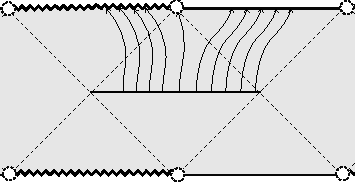
\includegraphics[width=1.05\textwidth]{SubextremalSchwarzschildDeSitterCongruence.pdf}
%% \put(-45,73){$\mathscr{I}^{+}$}
%% \put(-45,-8){$\mathscr{I}^{-}$}
%% \put(-75,30){$\tilde{\Sigma}$}
%% \end{figure}
%% \vspace{10mm}
%% %\end{block}
%% \end{columns}
%% \end{frame}





\begin{frame}
\frametitle{ ``Physical'' Killing Spinor ID}
\begin{columns}
\column{7.3cm}
\vspace{-5mm}
\begin{block}{Killing spinor}
  \begin{itemize}
  \item EFE: $\tilde{R}_{ab}=\lambda\tilde{g}_{ab}$ $\implies$ $\tilde{\Phi}_{AA'BB'}=0$
  \item $ \tilde{\nabla}_{A'(A}\tilde{\kappa}_{BC)}=0$
  \item $\tilde{\xi}_{a} \mapsto \tilde{\xi}_{AA'}:= \tilde{\nabla}^{B}{}_{A'}\tilde{\kappa}_{AB}$
    is a KV if EFE hold.
  \end{itemize}
\end{block}
\pause
\begin{exampleblock}{KSID zero-quantities definitions}
\vspace{-5mm}
\begin{subequations}
\begin{eqnarray*}
&& \tilde{H}_{A'ABC} := 3
  \tilde{\nabla}_{A'(A}\tilde{\kappa}_{BC)}, \label{DefZeroQuantityH}\\ && \tilde{S}_{AA'BB'}
  :=
  \tilde{\nabla}^{Q}{}_{A'}\tilde{H}_{B'Q AB}, \label{DefZeroQuantityS}
\end{eqnarray*}
\end{subequations}
\vspace{-6mm}
\begin{itemize}
\item $\exists$ Killing spinor %$\tilde{\kappa}_{AB}$
  %on  $(\tilde{\mathcal{M}},\tilde{\bmg})$
  $\iff$
  $\tilde{H}_{A'ABC}=0$.
\end{itemize}
\pause
\begin{multline*}\tilde{S}_{AA'BB'} = \tilde{\nabla}_{AA'}\tilde{\xi}_{BB'} +
  \tilde{\nabla}_{BB'}\tilde{\xi}_{AA'} \\ + 6\tilde{\kappa}_{(A}{}^{Q}\color{red}{\tilde{\Phi}}_{B)QA'B'}.
\end{multline*}
$\color{red}{\tilde{\bm\Phi}=0}$ \& $\tilde{\bmH}=0$ $\implies$ $\tilde{\bm\xi}$ is a Killing vector!
\end{exampleblock}
\column{4.3cm}
\vspace{-10mm}
\pause
\begin{block}{KSID (Valiente Kroon \& Garcia-Parrado 08) }
  \begin{itemize}
  \item Candidate KS eq for $\tilde{\bm\kappa}$, Candidate KV eq for $\tilde{\bm\xi}$.
  \item Assume $\color{red}{\tilde{\bm\Phi}=0}$.
  \item Closed system of homogeneous wave eqs
    \begin{eqnarray*}
    && \tilde{\square} \tilde{\bmH} = \mathcal{F}_{1}(\bmH,\bmS)\\
    && \tilde{\square} \tilde{\bmS} = \mathcal{F}_{2}(\bmH,\bmS)
    \end{eqnarray*}
    \vspace{-5mm}
  \item
    Trivial ID: $\tilde{\bmH}=\partial_t\tilde{\bmH}=\tilde{\bmS}=\partial_t\tilde{\bmS}=0$ on $\tilde{\Sigma}$, gives trivial solution
    $\bmH=\bmS=0$ on $\mathcal{W}\subseteq \mathcal{D}^{+}(\tilde{\Sigma})$
  \end{itemize}
\end{block}
\begin{alertblock}{KSID}
  $(\bm\tilde{\kappa},\partial_t\bm\tilde{\kappa})$ on $\tilde{\Sigma}$.
\end{alertblock}
\end{columns}
\end{frame}
%%%%%%%%%%%



%\begin{frame}{The conformal Einstein field equations}
\begin{frame}{The Einstein equations under conformal transformations}
\begin{itemize}
   \item The Einstein field equations in vacuum
     \vspace{-2mm}
\[
\tilde{R}_{ab} = \lambda \tilde{g}_{ab}
\]
 \vspace{-5mm}
 %\pause
 \begin{center}\large{\textbf{are not conformally invariant!}}.
 \end{center}
 \pause
\vspace{2mm}
\item A calculation shows that
\[
g_{ab} = \Omega^2 \tilde{g}_{ab}, \quad \implies
\]\vspace{-3mm}
\end{itemize}
\[
R_{ab} = \tilde{R}_{ab} -
\textcolor{red}{ 2\Omega^{-1} {\nabla}_a {\nabla}_b \Omega }
- {g}_{ab}\color{blue}{\big( \Omega^{-1} {\nabla}^c {\nabla}_c \Omega}
- \color{magenta}{3\Omega^{-2} {\nabla}_c \Omega {\nabla}^c \Omega\big)} ,
\]
where $R_{ab}$, $R$ and $\nabla_a$ are associated to
$g_{ab}$.
 \vspace{3mm}

\begin{itemize}
\item  \underline{Formally \textbf{singular}  whenever $\Omega=0$}!.
  \vspace{3mm}
  \pause
\item Friedrich's regularisation trick ... and  use the curvature as a variable
  \vspace{-2mm}
  \[ \textcolor{red}{{\nabla}_a {\nabla}_b \Omega}  = -\frac{\Omega}{2} {R}_{ab} + ...\]
  \vspace{-7mm}

\end{itemize}
\end{frame}


%%%%%%%%%%%

%\end{aligned*}
\begin{frame}{The conformal Einstein field equations (H. Friedrich 81)}
  \vspace{3mm}
\begin{columns}[c]
  \column{5.5cm}
  Equations:
  \vspace{-3mm}
\begin{flalign*}
%\begin{aligned*}
& {\nabla}_a {\nabla}_b \Omega = - \Omega {L}_{ab} + s g_{ab}, & \\
& {\nabla}_a s = -{L}_{ac} \nabla^c \Omega, \\
  & {\nabla}_c {L}_{db} - \nabla_d {L}_{cb}
  =d^a{}_{bcd} \nabla_a \Omega , & \\
  & {\nabla}_a d^a{}_{bcd} =0, &
 %\end{aligned*}
\end{flalign*}
\column{5.5cm}
\vspace{-2mm}
\begin{flalign*}
  %\begin{aligned*}
  & \text{Fields:} \quad (\Omega, s, L_{ab}, d^a{}_{bcd}) \\
& {L}_{ab} := \tfrac{1}{2} {R}_{ab}-\tfrac{1}{12} {R} {g}_{ab}, \hspace{2mm}  \mbox{\footnotesize{(Schouten tensor)}} \\
& s := \tfrac{1}{4} {\nabla}_a {\nabla}^a \Omega + \tfrac{1}{24}{R}\Omega, \hspace{2mm} \mbox{\footnotesize{(Friedrich scalar)}} \\
  & d^a{}_{bcd} := \Omega^{-1} C^a{}_{bcd}.  \hspace{2mm} \mbox{\footnotesize{(Rescaled  Weyl tensor)}}
   %& 6 \Omega s - 3\nabla_c \Omega \nabla^c \Omega =\lambda &
\end{flalign*}
\end{columns}
\vspace{3mm}
\begin{itemize}
  %\item  $$
  \vspace{-8mm}
%\item  Key equation: Rescaled Weyl spinor%No equation for $R$: Conformal gauge source function
%   \pause
\end{itemize}
\begin{block}{Key equation: Rescaled Weyl spinor}
  \begin{itemize}
    \vspace{-2mm}
    \begin{align}
     & \nabla^{AA'} \underbrace{(\Omega^{-1}\Psi_{ABCD})}_{\phi_{ABCD}\;\;\text{\tiny{rescaled Weyl spinor}}}
      = \Omega^{-1}\tilde{\nabla}^{AA'}  \Psi_{ABCD}  \underbrace{=0}_{\text{vaccum}\;\; \tilde{\Phi}=0} \nonumber \\
    & \boxed{\nabla^{AA'}\phi_{ABCD}=0} \qquad \qquad \Phi_{ABA'B'} \neq 0 \qquad \text{($\Phi$ sats diff eq)} \nonumber 
    \end{align}
 % \item Write $\bar{R}_{\mu\nu}$
    %   as second derivatives of the unphysical metric $\bar{g}_{ab}$.
    %\vspace{-5mm}
    % \item Frame approach: Use Cartan  structure equations.
    % Introduce: $\bme_{\bma}$, $\Gamma_{\bma}{}^{\bmc}{}_{\bmb}$
  \end{itemize}
\end{block}
\vspace{-5mm}
\begin{exampleblock}{Applications}
  \begin{itemize}
    \item Potentially turn {\bf{\emph{global}}} problems into {\bf{\emph{local}}} ones.
  \item $\mathscr{I}$ ($\Omega=0$) legit hypersurface to prescribe ID: Asympt. initial value problem. 
    \end{itemize}
  \end{exampleblock}
\end{frame}
%%%%%%%%%%%

\begin{frame}
  \frametitle{Combining these ideas?}
  \vspace{-3mm}
\begin{exampleblock}{Unphysical Killing vector equation}
Given a Killing vector $\tilde{\xi}^{a}$ on
$(\tilde{\mathcal{M}},\tilde{\bmg})$ and $(\mathcal{M},\bmg)$ with
$\bmg=\Omega^2\tilde{\bmg}$ then $X_{a}=\Omega^2\tilde{\xi}_{a}$
satisfies the \textbf{Unphysical Killing vector equations}
\begin{equation*}\label{ukve}
\nabla_{a}X_{b}+ \nabla_{b}X_{a}=\frac{1}{2}\nabla^{c}X_{c}g_{ab},
\quad X^{a}\nabla_{a}\Omega=\frac{1}{4}\nabla_{a}X^{a}.
\end{equation*}
\vspace{-5mm}
\end{exampleblock}
\vspace{-3mm}
\pause
\begin{columns}[c]
\column{5.5cm}
\begin{block}{ CKID: The conformal Killing vector initial data equations (Paetz 14)}
  \begin{itemize}
  \item Field equations: CEFE.
  \item  KID's on spacelike conformal boundaries $\mathscr{I}$ 
 % \item KID's on a spacelike 
  \end{itemize}
  \end{block}
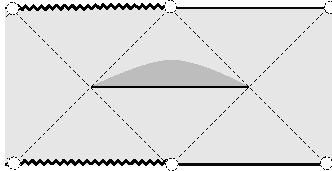
\includegraphics[width=1.00\textwidth]{figs/SdSIDphysical.pdf}
\put(-80,25){\large{$\color{black}\tilde{\Sigma}$}}

%\vspace{-3mm}
%\pause
\column{5.5cm}
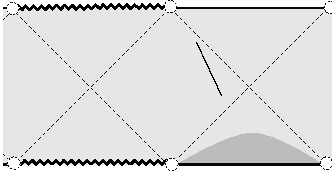
\includegraphics[width=1.00\textwidth]{figs/SdSIDunphysical.pdf}
\put(-54,-12){\large{$\color{black}\Sigma=\mathscr{I}$}}
\begin{block}{Apps \small{(Mars Paetz Senovilla 16, 17})}
  \begin{itemize}
    \item Characterisations of Kerr-de-Sitter-like spacetimes
    \end{itemize}
\end{block}  
\end{columns}
\end{frame}

%\section{The conformal Killing spinor initial data}

\begin{frame}
\frametitle{ CKSID Conformal Killing Spinor ID (G. \& Williams 22)}
\begin{columns}
\column{7.5cm}
\vspace{-7mm}
\begin{block}{ Killing spinors and conformal transformations}
  \begin{itemize}
  \item KS are
    conf. inv.
     $\tilde{\nabla}_{A'(A}\tilde{\kappa}_{BC)}=0$
    $\implies$ $\nabla_{A'(A}\kappa_{BC)}=0$
    with
    $\kappa_{AB}=\Omega^2\tilde{\kappa}_{AB}$.
  \end{itemize}
\end{block}
\pause
\vspace{-3mm}
\begin{alertblock}{Why proof doesn't work in conformal?!}
  \begin{itemize}
        %\item but ... %proof $(\mathcal{M},\bmg)$ doesn't work !
   \item The EFE are \textbf{not} conf. inv.
   \item $\xi_{a} \mapsto \xi_{AA'}:= \nabla^{B}{}_{A'}\kappa_{AB}$ is
     \textbf{not} a (C)KV.
  \end{itemize}
  \end{alertblock}
\vspace{-4mm}
\pause
\begin{exampleblock}{Zero-quantities?}
   \vspace{-2mm}
  \begin{align*}
  &H_{A'ABC}  := 3\nabla_{A'(A}\kappa_{BC)}\\
  & S_{AA'BB'}  :=\nabla^{Q}{}_{A'}H_{B'Q AB} \\ & \quad = \nabla_{AA'} \xi_{BB'} +
       \nabla_{BB'}\xi_{AA'} + 6\kappa_{(A}{}^{Q}\color{red}{{\Phi}}_{B)QA'B'}
  \end{align*}
  \vspace{-5mm}
     \begin{itemize}
   \item   $\bm\Phi$ satisfies diff conditions in $(\mathcal{M},\bmg)$.
   \item $\bmS$ not geom motivated.
   \item Relate $\bm\Phi$ to $\tilde{\bm\Phi}?$ $\leadsto$ Singular eqs $\Omega^{-1}$-terms
   \item Fuchsian systems theory vs CEFE philosophy
    %\item CEFE philosophy: avoid formally singular eqs.
     \end{itemize}
  \end{exampleblock}
\column{4cm}
\pause
\begin{block}{Buchdahl}
  %\begin{itemize}
  %\item
  $\bmH=0$ $\implies$  $(\mathcal{M},\bmg)$ Algebraically Special
    \begin{flalign*}
     & \nabla_{(A}{}^{A'}H_{\vert A'\vert BCD)} \\ & = 6 \kappa_{(A}{}^Q\Psi_{BCD)Q}=0
    \end{flalign*}
    Petrov Type D, N, O.
 $\Psi_{ABCD}=\Psi \kappa_{(AB}\kappa_{CD)}$
  % \end{itemize}
\end{block}
\begin{block}{Buchdahl zero-quantity }
  $\phi_{ABCD}=\Omega^{-1}\Psi_{ABCD}$\\
  \vspace{3mm}
  \textbf{Def Buchdahl 0-quant}
  \vspace{1mm}
  $B_{ABCD}:=\kappa_{(A}{}^Q\phi_{BCD)Q}$\\
  \vspace{3mm}
  $\nabla\times \bmH  = 6 \Omega \bmB$
\end{block}
\begin{block}{}
%%   \vspace{-5mm}
%% \begin{flalign*}
%%      & \nabla_{(A}{}^{A'}H_{\vert A'\vert BCD)}  = 6 \Omega B_{ABCD}
%% \end{flalign*}
\end{block}

\end{columns}
\end{frame}





\begin{frame}
\frametitle{  Conformal  (``Unphysical'') Killing Spinor ID}
\begin{columns}
\column{6.0cm}
\vspace{-4mm}
\begin{block}{Unphysical zero-quantities}
  \vspace{-5mm}
\begin{align*}
& H_{A'ABC}:=3\nabla_{A'(A}\kappa_{BC)}, \\
& B_{ABCD}:=\kappa_{(A}{}^Q\phi_{BCD)Q}.\\
  & F_{A'BCD}:=\nabla^Q{}_{A'}B_{QBCD}.
  \vspace{-3mm}
\end{align}
\end{block}
\vspace{-10mm}
\pause
\begin{exampleblock}{KSID (G. \& Williams 22) }
  \begin{itemize}
  \item Candidate KS eq for $\bm\kappa$.
  \item Assume vacuum CEFE are satisfied.
  \item Closed system of homogeneous wave eqs
    \begin{eqnarray*}
    && \square \bmH = \mathcal{G}_{1}(\bmH,\bmB)\\
    && \square \bmB = \mathcal{G}_{2}(\bmH,\bmB, \bmF)\\
   && \square \bmF = \mathcal{G}_{3}(\bmH,\bmB,\bmF)\\
    \end{eqnarray*}
    \vspace{-12mm}
  \item
    Trivial ID on $\Sigma$ %% $\bmH=\partial_t\bmH=0$ on $\Sigma$
    %% $\bmB=\partial_t\bmB=0$ on $\Sigma$\\
    %% $\bmF=\partial_t\bmF=0$ on $\Sigma$,
    $\implies$
    $\bmH=\bmB=\bmF=0$ on $\mathcal{W}\subseteq \mathcal{D}^{+}({\Sigma})$
    \item $(\bm\kappa,\partial_t \bm\kappa)$ on $\Sigma$.
  \end{itemize}
\end{exampleblock}
\column{5.8cm}
\vspace{-3mm}
\begin{block}{}
  \vspace{-5mm}
  \pause
\begin{equation*}
  \begin{array}{ll}
    \textcolor{black}{ \text{KS Candidate equation:}}
    \\ \\
	 \square \kappa_{AB} = -\frac{1}{6}R \;\kappa_{AB} + \Omega
         \phi_{ABCD}\kappa^{CD}
         \\ \\ \textcolor{black}{\text{Initial data on }} $\Sigma$:     
         \\ \\
         \kappa_{AB} =
         \mathring{\kappa}_{AB}
         \\ \nabla_{\bm\tau} \kappa_{AB}
         =  \mathcal{D}_{Q(A}\mathring{\kappa}_{B)}{}^Q
\end{array} 
\end{equation*}
\end{block}
\begin{block}{CKSID conds on $\textcolor{white}{ \Sigma}$}
  \begin{align*}
   & \mathcal{D}_{(AB}\mathring{\kappa}_{CD)}=0, \;\;
    \mathring{\kappa}_{(A}{}^Q\phi_{BCD)Q}=0
  \end{align*}  
\end{block}
\begin{block}{}
  $\mathcal{D}_{AB}$ is a Sen der intrinsic to $(\bmh,\Sigma)$
\end{block}
\end{columns}
\end{frame}
%%%%%%%%%%%

\begin{frame}
  
\begin{exampleblock}{Thm CKSID (G. \& Williams 22)}
  \begin{itemize}
  \item Given \textbf{ID for the vacuum CEFE}, if the CKSID conditions
  \begin{align*}
    \mathcal{D}_{(AB}\kappa_{CD)}=0, \qquad
    \kappa_{(A}{}^Q\phi_{BCD)Q}=0
  \end{align*}
  are satisfied on $\Sigma$,
  then there exists a Killing spinor
  in $\mathcal{W}\subseteq\mathcal{D}^{+}(\Sigma)$.
  \item
    In the asymptotic IVP set-up $\Sigma=\mathscr{I}$
    \end{itemize}
\end{exampleblock}
\vspace{-3mm}
\begin{center}
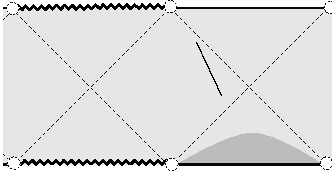
\includegraphics[width=0.8\textwidth]{figs/SdSIDunphysical.pdf}
\end{center}

\end{frame}



\begin{frame}
  \begin{columns}
    \column{6.0cm}
    \vspace{-4mm}
    \begin{exampleblock}{Corollary: Weyl collineation}
      \begin{itemize}
       \item  If $(\mathcal{M},\bmg)$ is a conformally Einstein manifold
       \item $\xi_{a} \mapsto \xi_{AA'}:= \nabla^{B}{}_{A'}\kappa_{AB}$ is a
         \textbf{curvature collineation} of the rescaled Weyl spinor:
      \item $\qquad \qquad \quad \mathcal{L}_{\bm\xi}\phi_{ABCD}=0$
      \end{itemize}
    \end{exampleblock}
    \vspace{-3mm}
    \begin{block}{Associated conformal Killing vector}
      \vspace{-3mm}
      \begin{equation*}\label{eq:conformalKillingVector}
  %X_a \mapsto
  X_{AA'}=\Omega \xi_{AA'} - 3 \kappa_{AQ}\nabla_{A'}{}^{Q}\Omega
      \end{equation*}
      \vspace{-5mm}
      \begin{itemize}
\item $X_a$ is a conformal KV of $(\mathcal{M},\bmg)$
\item $\tilde{X}_a=\Omega^{2}X_{a}$ is a KV of $(\tilde{\mathcal{M}},\tilde{\bmg})$
      \end{itemize}
      \pause
    \end{block}
    \begin{exampleblock}{Future applications}
      \begin{itemize}
    \item  Characterisation Kerr-de-Sitter through asympt ID.
    \item  Type D initial data characterisation.
      \end{itemize}
     \end{exampleblock}
    \column{4cm}
     \begin{block}{Future directions}
       \begin{itemize}
         
       \item Conds on a spacelike $\mathscr{I}$ for simplicity
       \item Other existence and uniqueness thms for wave eqs $\leadsto$
         \begin{itemize}
         \item Characteristic IVP
         \item IBVP
         \end{itemize}
         \item $\leadsto$ Data on null or timelike $\mathscr{I}$
\end{itemize}
     \end{block}
     \begin{center}
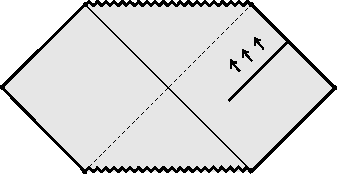
\includegraphics[width=1.1\textwidth]{figs/future2.pdf}
\end{center}
  \end{columns}
\end{frame}

\begin{frame}
  %  \vspace{2mm}
  \begin{center}
    \Huge{Many thanks for your attention}
    \end{center}

 \end{frame}

\end{document}








